\documentclass[12pt,a4paper]{article}
%\documentclass[review]{elsarticle}
\usepackage{lineno,hyperref}
\modulolinenumbers[5]
%\usepackage[numbers]{natbib}
%\usepackage{notoccite}

% Always needed
\usepackage{times}
\usepackage{parskip}
\usepackage{graphicx}
\usepackage{setspace}
\usepackage{url}
\usepackage{lscape}
\usepackage{multirow}
\usepackage{nameref,hyperref}
\bibliographystyle{unsrt}
\doublespacing
\raggedright


\begin{document}

\large {\bf Short-sighted evolution of Influenza cellular receptor binding avidity} \normalsize

Hsiang-Yu Yuan$^{1}$, James Hay$^{1}$, Katia Koelle$^{2}$

\begin{tabbing}
$^1$     \= MRC Centre for Outbreak Analysis and Disease Modelling \\
        \> Department of Infectious Disease Epidemiology \\
        \> School of Public Health \\
        \> Imperial College London \\
        \> London, United Kingdom \\ \\

$^2$    \> Department of Biology \\
            \> Duke University \\
            \> Durham, NC United States \\ \\
        

\end{tabbing}
\doublespacing
$^*$Corresponding author: Hsiang-Yu Yuan and Katia Koelle
\clearpage




{\bf Abstract}
Influenza viruses circulating in humans are known to undergo rapid antigenic evolution. These antigenic changes enable influenza to reinfect previously infected individuals within several years; as a result, seasonal influenza vaccine strains requires constant updating on a close to annual basis. Significant work remains, however, in understanding the selective drivers or the relevant factors of these evolutionary dynamics for planning and control of influenza outbreaks. Commonly, influenza’s antigenic drift is thought to arise from selection acting directly on drift variants. However, recent studies highlight the importance of frequent cellular binding avidity changes and deleterious mutations of influenza in evolutionary dynamics. \\
We extended a binding avidity hypothesis for influenza’s antigenic drift from serial passaging experiments to the population level through a combination of viral sequence analysis and simulation modeling. We demonstrated that net charge was a good marker of receptor binding avidity and it appeared to be a phenotype under immune-mediated selection in the human infection history. We constructed an individual based model incorporating immune history and within-host binding avidity adaptation. The model showed that while receptor binding adaptation enhances the length of the epidemic, the trait was under stabilizing selection in a heterogenous population, in which the binding avidity adapted within individuals towards either high or low binding avidity. This can be considered a case of ‘short-sighted’ evolution that decreases a virus’s effective reproductive number at the population level. Finally, a phylogenetic analysis of influenza H3N2 showed the consistent result that binding avidity was under stabilising selection. Together, we conclude that the adaptation of binding avidity within-host is short-sighted with regards to population fitness and that compensatory effects of binding avidity are important in eliciting antigenic jumps. 


{\bf Introduction}

% antigenic drift cause reinfection
Human seasonal influenza viruses reinfect human populations each year. One of the main reasons is that influenza viruses are known to undergo antigenic drift, a process by which amino acid substitutions occur in epitope regions of the viral hemagglutinin (HA) protein over time, resulting in the escape of host immunity induced from previous infection or vaccination. These antigenic changes enable influenza to reinfect previously infected individuals within several years; as a result, seasonal influenza vaccine strains requires constant updating on a close to annual basis (\cite{Carrat2007}). Understanding the factors driving antigenic drift is therefore critical for understanding patterns of disease incidence and for implementing effective influenza planning and control strategies. \\
% antigenic drift mechanism
In addition to the common thought that antigenic drift is a consequence of antibody selection acting on epitope regions (\cite{Grenfell2004} \cite{Wilson1990}), the hypothesis that antigenic drift could also be driven by frequent alterations of HA binding avidity was proposed, inspired from observations from the serial passaging of the virus in mice (\cite{Hensley2009}). According to the mouse experiments, the cellular receptor binding avidity of HA increased when the virus was passaged to immune mice and decreased when passaged to naive mice. Because a large proportion of the binding avidity mutations are located in the epitope domain, antigenicity would likely be altered as a byproduct of binding avidity mutations. Consequently, antigenic drift could be driven by frequent HA binding avidity changes during disease transmission in a heterogenous population with different levels of immunity. Vaccination targeting children was proposed to reduce the antigenic drift rate by minimizing immune heterogeneity in a population. Our previous simulation also confirmed the effect of vaccination on lowering antigenic drift by targeting naive individuals (\cite{Yuan2013}). \\
% Current challenges in antigenic drift mechanism
However, challenges exist in projecting the mechanism of binding avidity changes in mice serial passaging experiments on to disease transmission in the human population. First, despite the evidence for binding avidity adaptation in mice, there is currently a lack of population studies that demonstrate influenza viruses binding avidity adaptation to heterogeneous immunity in humans. Second, serial passaging studies allow immune hosts to be infected through injection with high viral dosage, whereas  the stringency of bottlenecks during the natural transmission of the virus (\cite{Varble2014}) results in the low likelihood for virus transmission to hosts with strong immunity  Third, in the passaging studies, finely scaled immunity and its corresponding clinical protection, like that which exists in a natural human population, is ignored (\cite{Yuan2016}). The heterogeneities in population immunity would affect the fitness of the binding avidity mutations and produce differences in disease transmission. With continually changing immunity in the population during epidemics, the effects of receptor binding mutations in epidemiological and evolutionary dynamics would therefore vary accordingly. Furthermore, although higher binding mutations enable viruses to escape from pre-existing immunity, lower fitness of these mutations was observed when viruses were re-passaged into naive mice. This indicates that the mutations with higher binding avidity could possess additional costs or harmful effects when the viruses replicate in individuals with lower immunity. Recent studies have demonstrated that mutations with deleterious effects would be important factors that affect the fitness of strains (\cite{Luksza2014}) and their evolution (\cite{Koelle2015}). Together, a greater understanding of the evolution of receptor binding avidity in a human population with changing immunity is essential for understanding patterns of disease incidence and for implementing effective influenza vaccination strategies. \\
To understand how virus binding avidity evolves and its impact on disease transmission, we first demonstrated that the binding avidity adaptation was likely present in human population by comparing the marker of binding avidity to antibody prevalence. We also developed an individual-based model linking within-host virus evolution to population level disease transmission, coupled with individual host immune response. The continuous scale of the immunity and their corresponding clinical protection, like that which existed in a natural human population, were included. We demonstrated that short-sighted evolution existed such that the viral lineages with less variability would persist longer during the epidemic, indicating the deleterious effects of frequent changes of binding avidity.  Finally, phylogenetic analysis of public influenza virus sequences was performed and supported the hypothesis that  binding avidity of human influenza viruses evolve in a short-sighted manner. \\
\clearpage



{\bf Results}

%1. Net charge is a good marker of binding avidity
{\it  Net charge appears to be a good marker of binding avidity} \\
Net charge of HA appeared to be a good marker for receptor binding avidity of influenza viruses.  Since there are no large scale systematic studies on binding avidity of different viral mutants, in order to evaluate whether the adaptations of the binding avidity to host immunity can be observed within human influenza infection history, we first investigated whether changes of net charge of HA can be used as molecular markers for binding avidity since net charge is considered to affect receptor binding avidity (\cite{Arinaminpathy2010}). Because the sialic acid receptor on host cells has a negative net charge, such that a more positive net charge of the viral HA is likely to increase the electrostatic force between the viral HA and its sialic acid receptor. We collected publicly available amino acid substitution data with corresponding receptor-destroying enzyme (RDE) activities from the literature and grouped them  according to whether the amino acid substitutions reduce (negative), maintain (neutral), or increase (positive) the net charge. Interestingly, the largest increase of binding avidity was among the positive amino acid group and the lowest increase was among the negative group (\nameref{Fig1}).  We also observed that the substitutions which have higher net charge enhanced binding avidity significantly comparing to the mutations which reduced net charge (p value = 0.0001; TableS1), suggesting that net charge appeared to be a good marker for HA binding avidity. A significant correlation also occurred when the binding avidity was compared to the absolute net charge using the HA sequences (FigureS1). \\

%2. Net charge correlates to seroprevalence
{\it  Net charge correlates to seroprevalence} \\
The age distribution of net charge supported the presence of binding avidity adaptation in human infections. We collected influenza H3N2 sequences with infected persons’ age metadata isolated from 1994-2005 as part of an Influenza Genome Sequencing Project  [20]. The percentage of the viruses having a high absolute net charge (defined as an absolute net charge greater than the median value of 18) followed a V-shaped distribution by age. The valley of the distribution occurred in persons between 40-60 years old (yo) and the two peaks occurred in the age groups 0-20 and 60-80 yo (\nameref{Fig2}). The net charge distribution of different age groups from these human virus isolates was compared to the age specific serological prevalence. Interestingly, the antibody responses by age against the H3N2 strains from 1995 to 2005 also showed a similar V-shaped distribution, with two maximums in young adults and the elderly, and the minimum between 40-60 yo (\cite{Kucharski2015a} \cite{Kucharski2012}). The congruent V-shaped age distributions that were observed from both the net charge of the isolated viruses and the population immunity along with the significant correlation between net charge and binding avidity supported the hypothesis that a higher binding avidity could be selected for by higher host immunity in a human population  (\cite{Hensley2009}), indicating the presence of binding avidity adaptation in human influenza history.  \\

%3. We constructed a model to study the Effect of Binding Avidity Adaptation 
{\it  a model to study the effect of binding avidity adaptation } \\
To understand the impact of influenza binding avidity on epidemic dynamics, we constructed an individual-based epidemic model, coupled with within-host binding avidity adaptation (\cite{Hensley2009} \cite{Yuan2013}) and individual antibody responses (\cite{Yuan2016}). Within each infected individual, the virus binding avidity adapted to host immunity and reached a higher fitness as defined by the within-host reproductive number $R_{in}$ (\nameref{Fig3} A). Different levels of host immunity were mapped to the corresponding susceptibility (defined as the probability of infection given a contact) as a function of  virus binding avidity. In our model, a higher host immunity reduces the probability of infection and results in  a higher optimum binding avidity through escaping host immunity (\nameref{Fig3} B). To measure the impact of binding avidity during the epidemics, we first simulated transient disease dynamics by introducing one antigenic mutant strain into a heterogeneous population with pre-existing partial immunity. \\

%4. Binding Avidity Adaptation prolong the incidence curve 
{\it  Binding avidity adaptation prolong the incidence curve } \\
Our simulation results demonstrated that the within-host binding avidity adaptation prolongs the epidemic period. After the seeding viruses were introduced with a low initial binding avidity, peak incidence was achieved after approximately 200 days (\nameref{Fig4}). During the outbreak, the increase of the binding avidity was correlated with the increase of average population immunity. The number of naive individuals (defined as pairwise immunity level = 0) dropped as successful infections increased the level of immunity in the population (\nameref{Fig5}).  The number of individuals with higher immunity increased rapidly as the incidence approached the maximum peak, during which a greater amount of antibody boosting would be produced. The average binding avidity was near 0.45 in the early phase (when different initial binding avidities were used, the avidities quickly adapted to near 0.45 before the incidence peak) of the epidemic and later increased to around 0.6 to adapt to the higher immunity population in the late phase. We compared this result to the scenario with binding avidity that was fixed to the early adapted and the late adapted values. The adaptation of binding avidity prolonged the incidence curve until it faded out and produced a larger incidence comparing to the scenario with binding avidity fixed to the early-phase adapted binding avidity. Interestingly, the maximum incidence produced by the adaptation of binding avidity was lower than scenario with binding avidity fixed to the late-phase adapted binding avidity t, indicating the detrimental effects of binding avidity adaptation on disease transmission.  \\

%5. Binding avidity adaptation are deleterious
{\it  Binding avidity adaptation are deleterious } \\
Within-host binding avidity adaptation produced a deleterious effect on disease transmission in the population. To understand why within host binding avidity adaptation produce a lower incidence than the viruses whose binding avidity fixed at the adapted value, we calculated the optimum binding avidity at the population level by time along with the changes in population immunity over the course of the outbreak. The optimum binding avidity is defined as the avidity at which the greatest number of viral offspring can be produced, as measured by the effective reproductive number $R_{t}$. During the outbreak, the average binding avidity among infected individuals before within-host adaptation (at the time of infection) was lower than the population optimum binding avidity. Furthermore, the average adapted binding avidity after within-host adaptation (at the end of the infection period) was even further away than the optimum binding avidity and produced an even lower $R_{t}$ (\nameref{Fig6}). This demonstrated that within-host binding avidity adaptation appeared to lower population-level fitness relative to the population-level optimum. \\

%6. Short-sighted evolution binding mutations can be explained by the differences among within- and between-host selection
{\it  Short-sighted evolution of binding mutations } \\
Within-host binding avidity evolution was short-sighted in a population with partial immunity. To understand why the binding avidity adapted to a suboptimal fitness, we compared the within host adaptation of viral traits to the population level fitness with different antigenic changes at different stages of the outbreak. Given the distribution of individual immunity, we first calculated the possible evolutionary outcome of a viral mutant. During disease transmission in a population, the chance of the viral mutant surviving depends on the evolutionary fitness from both within-host selection ($R_{in}$) and between-host selection ($R_{t}$). \\
When a strain with a random mutation (occurred at one or more than one amino acid site) in the binding avidity trait was introduced in a partially protected population, the average relative probability of this mutation being reproduced within infected individuals was approximately a linear curve decreasing monotonically with binding avidity regardless of the magnitude of antigenicity change (\nameref{Fig7}). Without or with only moderate antigenic changes, this distribution contradicted the between-host selection at the population level, as the population fitness tended to be optimal at a higher binding avidity during the outbreak (\nameref{Fig7}). Thus, although lower binding avidity mutations were more likely to be reproduced within naive individuals, the short-sighted within-host evolution resulted in a deleterious effect at the population level since the probability of infection by viruses with low binding to the persons with partial immunity was low (\nameref{Fig3} B). The accumulated herd immunity through depletion of susceptibles during the epidemics increased the deleterious effects of within-host binding adaptation (FigureS2). When the antigenicity change became strong such that all the individuals became naive, then low binding avidity mutations would produce an optimal fitness on both within-host and population levels through the compensatory effect. \\

%7. The Deleterious Effect of Binding Avidity Adaptation on viral phylogeny
{\it  Analysis of simulated viral phylogeny} \\
The deleterious effect of adaptive binding avidity was further demonstrated by comparing the binding values at the internal and external nodes of the viral phylogeny constructed from our individual based simulation. When binding avidity adaptation was present, many of  the ‘mutants’ which adapted to very low binding avidity were present as external tips (\nameref{Fig8}). However, the viruses that were present in internal nodes (more likely to produce more offspring in the population), displayed a limited range of binding avidities between the average binding avidity at external tips and the population optimum binding avidity. This was due to the balance of the selection force from the within-host adaptation and the total population. To verify the deleterious effect of binding avidity on transmission, we adjusted the probability of infecting hosts with different levels of immunity to be less differential and more uniform, as would be the case in a serial passaging experiment without deleterious effects. In this case, the viral phylogeny showed a more homogenous probability distribution of binding avidities at internal and external nodes (FigureS3). This suggested that the deleterious effects were caused by differential selection due to the change of the immune profile in the population. \\

We further simulated the influenza dynamics with antigenic drift across multiple years. We specify the probability of the occurrence of the random mutation and the effect of its antigenicity change (TableS3). When binding avidity was fixed, a balanced tree with multiple lineages would be produced (\nameref{Fig9}). Interestingly, when binding avidity was allowed to be adapted to the individual immunity, a ladder liked tree was generated.     

%8. Phylogenetic Analysis
{\it  Phylogenetic analysis} \\
The larger variation of net charge present in the external than internal nodes in the reconstructed phylogenetic tree support the short-sighted evolution of binding avidity. To test whether the predicted deleterious effects can actually be seen in influenza H3N2 infection history, we collected viral sequences isolated from North America and reconstructed the ancestral state of the nucleotide. We observed net charge changes between different clades, but in each clade, we did not observe frequent sequential alterations within the clades (\nameref{Fig10} A). Although the net charge trait was widely distributed within each year, when the strains were grouped by the number of glycosylation binding sites (which could possibly affect the binding avidity), the net charge maintain a very narrow variance in the trunk and other internal nodes (\nameref{Fig10} B). For all internal nodes, only $7.7\%$ of the strains showed net charge change; whereas in external tips, which were destined to soon die out, a higher proportion of the strains ($12.1\%$) demonstrated changes in net charge (TableS3). A lower average net charge with a higher variance were seen at external tips (17.45 $ \pm1.18$) than internal nodes (17.52 $ \pm1.19$), consistent with the simulated phylogeny from our model (\nameref{Fig8}). Internal nodes also demonstrated a higher proportion of high net charge, indicating better adaptation to partially protected populations than external strains. \\

\clearpage

{\bf Discussions}
\textit{} \\
% Summary
We have demonstrated that influenza net charge is significantly correlated with binding avidity. We observed similar patterns in the fraction of high net charge viral strains and human seroprevalence, indicating that adaptation of influenza binding avidity to herd immunity in human population is likely present. We have developed an individual-based epidemic model incorporating within-host virus binding avidity adaptation, individual immune boosting and host infection histories. The model allows us to produce a simulated viral phylogeny and to observe changes of virus characteristics (such as antigenic change and binding avidity) along with the changes in individual host immunity over time. The model predicts short-sighted evolution of binding avidity: First, the binding avidity after within-host adaptation would lower the reproductive number compared to that before within-host adaptation. Second, low binding avidity in naive individuals could lower population-level fitness due to the deleterious effects of low binding avidity in a population with partial protection. Third, the external nodes, which become extinct, demonstrate larger net charge variation and lower average net charge. A similar observation was found in the influenza H3N2 phylogenetic tree, which displays lower net charge variation along internal lineages and a lower absolute net charge in external tips. \\
%Short sight evolution of binding avidity within-host adaptation
We demonstrated that within host viral binding avidity adaptation would ‘produce’ deleterious mutations. Based on the observation of within-host adaptation in serial passaging experiments,  we linked the within-host mechanism to the human population, in which differential susceptibility caused by partial immunity would need to be considered. With partial immunity, we did not observe significant alternative changes in net charge among viral lineages in a single season or a clade in our phylogenetic analysis nor from our model simulation, which were required to continually drive antigenicity change as a by-product of binding avidity change. This is because within-host adaptation of binding avidity is demonstrated to be short-sighted in a heterogenous population, such that the average binding avidity at the end of the infectious period evolves further away from the optimum binding avidity compared to the binding avidity at the beginning of the infectious period, resulting a further reduction in reproductive number. For example, when influenza virus binding avidity decreases once a naive host is infected, the low binding avidity could become deleterious during the epidemics in a population with partial immunity. The short-sighted within-host evolution has also been predicted in other RNA viruses such as HIV (\cite{Lythgoe2013}). Once within-host competition increases, HIV evolves to higher virulence; however, the fitness of the viral population at the epidemiological level decreases. For influenza, the more viruses that adapt to either naive individuals or those with strong immunity, the lower the fitness that would be produced in a  heterogeneous population. \\
%Antigenic drift could be driven by binding avidity change as Compensatory mutation 
Although we observed that average virus binding avidity maintains a more stabilized level in internal nodes than external tips within a season,  the average binding avidity between the seasons changes. The increase in binding avidity between seasons could be a result of adaptation to an increased herd immunity, whereas the decrease in binding avidity between seasons could be caused by compensatory binding mutations accompanied by large scale antigenic changes. When an antigenic mutation occurs with a large effect, optimum binding avidity adaptation would produce a higher fitness through compensatory effects, which can explain that the major substitutions in influenza history are located in receptor binding sites (\cite{Burke2013}). \\
%Binding avidity prolong the length of the incidence 
This study raises a fundamental question regarding the effects of binding avidity adaptation in influenza evolution: why do influenza viruses adopt a strategy that lengthens survival time of virus lineages to “wait” for a novel antigenic variant rather than simply increasing the rate of incidence? Our results are consistent with several assumptions that have been made to support a short-sighted evolution hypothesis including within-host evolution towards a higher virulence or to escape from the immune system’s recognition. (\cite{Levin1994}). However, here we also demonstrated that binding avidity evolution, even though short-sighted, could potentially reduce the probability of virus extinction. \\
%Future challenges
Due to the short-sighted evolution, optimal vaccination strategies becomes more difficult to understand than previously thought. A vaccination strategy that might reduce transmission events in a heterogenous population is to immunize  individuals with only partial protection due to the differential selection. In a population with partial herd immunity, multiple antigenic strains would likely co-exist together before one final antigenic strain replaces others and becomes dominant. Among them, the one with optimum compensatory mutations on binding avidity that would increase transmissibility most is likely to become the progenitor of the future antigenic strain. Therefore, this study highlights the need to incorporate binding avidity change in addition to serological titres to select or predict possible future vaccine strains. To understand the effect of binding avidity on disease dynamics and transmissibility and the evolutionary strategy of binding avidity of the virus would be beneficial for future antigenic strain prediction. \\
\clearpage


{\bf Material \& Methods}

\textit{Analysis of HA cellular receptor binding avidity} \\
The RDE binding avidity for amino acid changes were collected from the literature (\cite{Hensley2009} \cite{Das2011} \cite{Myers2013} \cite{Li2013a}) and also obtained directly from the group performing the RDE assays(\cite{Hensley2009}). In total, 74 mutants were collected, including 53 single, 20 double and 1 triple amino acid changes. For the RDE binding avidity assay present in the literature, the magnitude of each change was extracted using the Web Plot Digitizer(\cite{Rohatgi2012}). The effect of each single amino acid change on binding avidity was calculated as the log ratio of RDE activity of the mutant compared to the wild type (TableS2 and TableS3).

\textit{Calculating net charge of influenza HA} \\
Influenza virus sequences isolated from New York State as part of the Influenza Genome Sequencing Project (\cite{Ghedin2005}) along with the exact date of isolation and clinical metadata on host age were collected from the Influenza Virus Resource Database (\cite{Bao2008}). We obtained in a total of 686 full-length influenza A/H3N2 HA sequences isolated between 1993 and 2005. Changes in net charge were estimated by summing the total number of positively charged amino acids minus the number of negatively charged amino acids. Amino acid such as Arginine (R), Histidine (H) and Lysine (K) are positively charged whereas Aspartic acid (E) and Glutamic acid (D) are negatively charged. For estimating net charge from the isolated viral HA sequences, net charge was calculated from the sequences using amino acid positions 17 through 345 of the HA, which define the protein’s globular head domain (HA1). We specifically did not calculate net charge values using only the amino acid positions that comprise the cellular receptor binding site because charge at other sites in the globular head domain also impact electrostatic forces and thereby binding avidity. \\
\textit{Phylogenetic Analysis} \\
Phylogenetic trees were reconstructed using the software program BEAST (\cite{Drummond2012}), under a general time reversible (GTR) model with gamma distributed rate variation and a proportion of invariant sites. $10^{7}$ MCMC steps were sufficient in reaching a high effective sample size. From each viral subtype’s maximum clade credibility (MCC) tree, we inferred the ancestral states of the observed viral sequences. If BEAST produced multiple possible ancestor sequences, consensus sequences were calculated with BLOSUM50 scoring matrix using Matlab Bioinformatics Toolbox. For all the observed external and inferred internal sequences we calculated net charge as described above.

\textit{The Individual based modelling} \\
We developed an individual based model in which individual hosts could be susceptible ($S$), infected ($I$) or recovered ($R$) with respect to infection. Individuals also had varying immune states, $K$, which was defined as the magnitude of specific immunity against the first antigenic strain in individuals’ infection history(FigureS4). We considered each virus individually at the population level, allowing us to track the identity of each infected host as well as certain virus characteristics such as antigenic distance, $\delta$, and binding avidity, $V$.

The model was simulated under demographic stochasticity using Gillespie’s tau-leap algorithm (\cite{Gillespie2001}) to calculate the probability of events occurring for each individual in each day. We assumed that births of new hosts occurred at a rate 1/70 per year, and that each new host began with a completely naive immunity ($K = 0$). Similarly, deaths occurred at the same rate for the entire population thereby ensuring a constant population size. Total number of contacts was calculated based on the contact rate c, number of susceptibles X, and number of infecteds Y in a population of size N, resulting in cXY/N total contacts per unit time. As shown in FigureS4, for each contact, a random susceptible target $S_{tar}$ and an infected source $I_{src}$ were drawn from the population. The probability of successful transmission, $\rho$, was determined by the effective immunity $J$ of the target host (see the following sections for calculating $\rho$) against the challenging source virus $v_{i}$, and the binding avidity $V$ of the virus at the time of contact (FigureS4B). Effective immunity $J$, was defined as the magnitude of the host immune status $K$ minus the shortest antigenic distance between the challenging virus $v_{i}$ and the past infected strains in the host’s infection history $h$, $J =K - min(\delta_{ih})$. The antigenic distance can be derived by tracing back along the transmission tree to find the most recent common ancestor of the infecting virus $v_{i}$ and the infection history viruses $h$ and calculate the sum of all each individual antigenic changes along this the path $\delta_{ih}$.

Once an individual became infected, the average infectious period $1/\gamma$ lasted 3.3 days, during which the virus’ binding avidity $V$ adapted to the host immunity $J$ at a rate determined by the fitness gradient (figure3A \cite{Yuan2013}). After the infected individual recovered, the individual became transiently fully protected for an average of 25 days ($1/\omega$) through short-lived immunity, possibly mediated by cytotoxic T lymphocytes along with other immunological factors (\cite{Ferguson2003} \cite{Kaech2012}). During the recovered period, individual immune state $K$ was boosted following a Poisson distribution with mean $g=3$. After transient immunity waned, the recovered individual became susceptible again but with protection from subsequent viral infection through increased effective immunity $J$.

\textit{Probability of infection} \\
Each time a virus $v$ came into contact with a susceptible host $S$, the probability of successfully infecting that host was defined as the 1 minus the probability of stochastic extinction of the viruses within that host:

$\rho = \frac{1}{1-(R_{in})^\sigma}$

where $R_{in}$ is the reproductive number in a host and $\sigma$ is the number of viruses initially transmitted. $R_{in}$ was defined as the expected number of virions produced by a single virus in a host with effective immunity $J$:

$R_{in}=n \cdot f(J,V) \cdot g(V)$

Where $f(J,V) = [1 - e^{p(V+1)}]^r$ and $J$ is the probability of evading the immune response with a given virus binding avidity $V$, and a given host immunity $J$ ;  and $p$ and $r$ are scaling constants. $g(V) = e^{(aV^b)}$is the probability of successful replication within a host with a given binding avidity $V$, where $a$ and $b$ are scaling constants (\cite{Yuan2013}). Combining these probabilities with the average number of offspring $n$ produced after the replication by a single virus gives the reproductive number for viruses within a host.

\textit{Within host adaptation and antigenicity change} \\
During the infectious period, binding avidity $V$ of each infection strain adapted to the host’s immunity $J$. The change of binding avidity $\Delta V(t)$ was defined as the product of the rate of change of the virus binding avidity $dV/dt =V_{c}(dR_{in}/dV)$ and the time since infection $\Delta t$ (\cite{Yuan2013}), where $V$ is the within-host binding avidity of the virus, $dR_{in}/dV$ is the fitness gradient, and $V_{c}=0.075$. We considered the scenario where antigenic drift occurred as sum of the epitope changes that contain both randomly produced antigenic mutations, which complies with the classical hypothesis of antibody selected antigenicity changes, and the mutations produced as a byproduct of binding avidity change. Random antigenic mutations occurred with a probability $\psi$, and the effect of the antigenic change $\kappa_{a}$ was drawn from an exponential distribution with average antigenic distance. Changes in binding avidity also translated into small changes in antigenicity described by parameter $\kappa_{b}$, such that rate of antigenic change due to binding avidity change was proportional to the rate of change of binding avidity (parameter values were listed as TableS4). Therefore the total antigenic change which occurred in the virus during an infection was expected to be

$\delta =\kappa_{a} \psi+\kappa_{b} \Delta V.$

\textit{Initial population immunity} \\
We began each simulation using initial conditions for the immune profile of susceptible individuals produced after a single epidemic peak. To match the distribution of partial immunity that was observed in a population, we ran the simulation from a completely naive population to generate a distribution of host immunities. The epidemics generated a total incidence of roughly 50\%. Each infected individual received a boost to immunity drawn from a Poisson distribution with mean $g=3$, resulting in a distribution of host immune states, $K$. All simulations were then run using the same host immunity distribution, $S_{k}$, introducing a new virus with antigenic distance $\delta =2$ relative to the strain used for the generation of initial conditions. The resulting overall distribution of $J$ was similar to serological data for seasonal influenza (\cite{Yuan2016}).

\textit{The fitness in a changing immune profile environment} \\
The effective reproductive number was calculated whilst taking into account the changing total number and immune profiles of susceptible individuals over time. Given a single virus with binding avidity V, the effective reproductive number given time $t$ was defined as:

\begin{equation}
R_{t}=\frac{\sum_{J=0}^{\infty}\beta(J,V)S_{t}(J)}{\gamma N}
\end{equation}

The average within host relative fitness $\bar{w}$ of a virus with a particular trait was calculated using the immune profiles of susceptible individuals at time $t$. We first calculated the normalized frequency of the newly infected individuals in which the virus would be replicated in as:
\begin{equation}
I_{t}^*(J,V)=\frac{\beta(J,V) S_{t}(J) }{\sum \beta(J,V)\ S_{t}(J)}
\end{equation}

Under the assumption that the fixation probability of a mutation is proportional to its within-host fitness in infected individuals (\cite{Gillespie1984}), we calculated the average within host relative fitness $w$, given by
\begin{equation}
\bar{w}_{t}(V)=\frac{\sum_{J=0}^{\infty} R_{in}(J,V)I_{t}^*(J,V)}{\max{R_{in}(J,V)}}
\end{equation}
\clearpage

{\bf Figure Legends} \\

\includegraphics[width=1\textwidth]{fig/png/Figure1.png}
\paragraph*{Figure1.}
\label{Fig1}
Binding avidity change of single amino acid mutations by net charge. The value is calculated as the log ratio of RDE activity of the mutant to that of the wild type. Amino acid mutations are grouped in 3 categories. Increase represents amino acid changes that increase net charge by 1 or 2 units. Decrease represents the amino acid changes that decrease net charge by 1 or 2 units. Same represents net charge is same. Aspartate (D), glutamate (E) are counted as negatively charged amino acids (-1) and Histidine (H), Arginine (R), Lysine (K) are counted as positively charged (+1).
\clearpage


\includegraphics[width=1\textwidth]{fig/png/Figure2.png} 
\paragraph*{Figure2.}
\label{Fig2}
Net charge distribution by age group. The proportion of higher net charge is calculated for 5 age groups (0-19, 20-39, 40-59, 60-79 and $\geq80$). Virus sequences and clinical data are obtained from the Influenza Genome Sequencing Project (\cite{Ghedin2005}) and the Influenza Virus Resource Database (\cite{Bao2008}). 
\clearpage

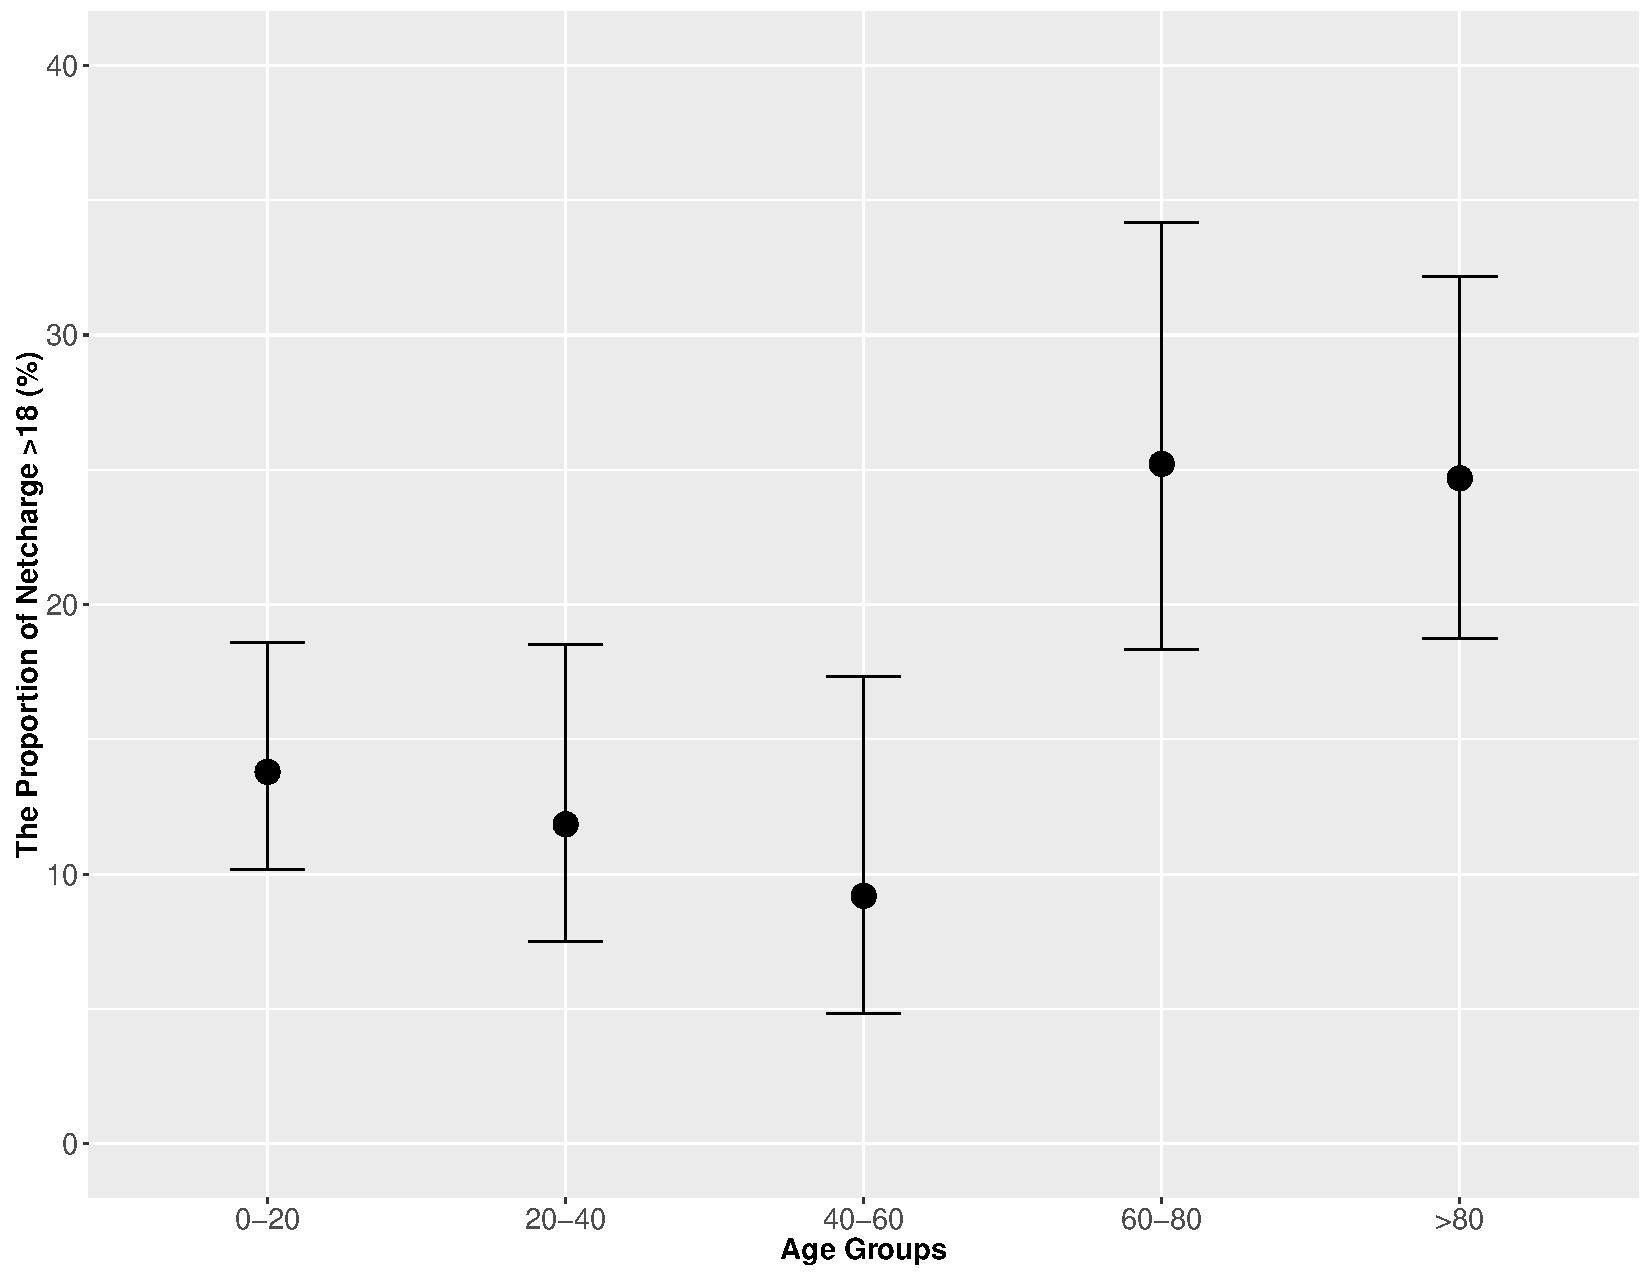
\includegraphics[width=0.6\textwidth]{fig/png/figure3.png}
\paragraph*{Figure3.}
\label{Fig3}
Within host reproductive number and the probability of infection. (A) Within-host fitness represented by the expected within-host reproductive number $R_{in}$. Parameters for within-host immune escape and replication cost were set as p=4, r=70, a=0.7 and b=3, and virus offspring number was set to $n=4$ (see Methods section for parameter descriptions). Bluer colours indicate more immunologically naive individuals, whereas redder colours indicate higher immunity individuals. (B) The probability of infection with differential selection. Within-host parameters values are same as (A) and the effective initial number of transmitted virions was $\sigma$=1. (C) The probability of infection with weak differential selection. Parameter values same as (A) but the effective initial number of the transmitted virions was $\sigma$=3 to represent a higher viral dosage as would be the case in serial passaging transmission.
\clearpage

\includegraphics[width=1\textwidth]{fig/png/figure4.png}
\paragraph*{Figure4.}
\label{Fig4}
Simulated epidemic with and without within-host binding avidity adaptation. An antigenic strain with $\delta=2$ was introduced without continual antigenic drift during the epidemics, $\kappa_{a}=0$ and $\kappa_{b}=0$. The red line shows the incidence when binding avidity is allowed to adapt within hosts over the course of the epidemic, starting at a binding avidity of V=0.45. The blue line shows incidence when binding avidity is fixed near the late stage population average of V=0.6, eliciting a rapid, large peak. The green line shows the incidence when binding avidity is fixed near the early phase population average at $V=0.45$, resulting in a very small epidemic peak. In all scenarios, Total population $N$ is set to be 1,000,000. For the initial day, the number of seed viruses $I_{0} = 100$, recovered hosts $R$ = 0 and the remaining hosts were susceptible under the initial immunity distribution as described in the Methods. The remaining epidemiological parameters were described in TableS4. Within host parameters were as described in FigureS1.
\clearpage

\includegraphics[width=1\textwidth]{fig/png/figure5.png}
\paragraph*{Figure5.}
\label{Fig5}
Distribution of population immunity during the epidemic with binding avidity adaptation. Colours show the proportion of susceptible hosts with a given level of effective immunity against the seed virus, J, over time. The white line represents the population mean immunity level. At the start of the simulation, the majority of hosts are completely naive to the novel strain, with some hosts exhibiting low levels of immunity due to prior infection. As incidence increases, the mean host immunity also increases as infected hosts recover and develop long-term immunity. This coincides with the peak of incidence at around 200 days. Parameters are as described in \nameref{Fig3} and \nameref{Fig4}.
\clearpage

\includegraphics[width=1\textwidth]{fig/png/figure6.png}
\paragraph*{Figure6.}
\label{Fig6}
The effective reproductive number by time and binding avidity. The effective reproductive number was calculated against the population contained only susceptible individuals with differential protection (as in \nameref{Fig5}) but excluding the transiently recovered and infected individuals. The optimum binding avidity (dotted line) is that which produces the largest number of offspring at the population level. The effective reproductive number produced by the optimum binding avidity was projected to the bold gray line. Red, the mean binding avidity across all extant virions at the start of the infectious period. Light blue, the mean final binding avidity across all extant virions at the end of the infectious period. Bold gray, the optimum reproductive number. Thin gray, the effective reproductive number when binding avidity is fixed at 0.
\clearpage

\includegraphics[width=1\textwidth]{fig/png/figure7.png}
\paragraph*{Figure7.}
\label{Fig7}
Within-host and between-host relative fitness by binding avidity and antigenic change. Within-host relative fitness is shown by the red surface. Between-host relative fitness is shown by the  surface ranging from blue (low) to yellow (high) to represent the value from low to high.
\clearpage

\includegraphics[width=1\textwidth]{fig/png/figure8.png}
\paragraph*{Figure8.}
\label{Fig8}
The deleterious effect of within-host binding avidity adaptation on viral phylogeny . Blue dots represent internal nodes from the viral phylogeny. Green dots represent external tips from the viral phylogeny. The dotted line shows the optimum virus binding avidity that will produce the greatest number of offspring at the population level. Bold gray represents mean binding avidity from internal nodes. Light gray represents mean binding avidity from external nodes Parameter values were as described in \nameref{Fig3}A and B.
\clearpage

\includegraphics[width=1\textwidth]{fig/png/newfigure10.png}
\paragraph*{Figure9.}
\label{Fig9}
Simulated viral phylogenies with and without binding avidity adaptation. (A) Influenza phylogeny with fixed binding avidity adaptation. (B) Influenza phylogeny with binding avidity changes.


\includegraphics[width=1\textwidth]{fig/png/figure9.png}
\paragraph*{Figure10.}
\label{Fig10}
Phylogenetic  analysis  of cellular receptor binding avidity. (A) The maximum clade credibility (MCC) tree for the H3N2 viral isolates from New York State, with HA net charge values mapped onto all inferred internal nodes and all observed external nodes. Numbers next to the bracketed clades denote the $\#NGS$ group. (B) Viral net charge dynamics over time. Each point represents a node from (A) and is colored by whether it is classified as an internal trunk node (red circle), an internal non-trunk node (blue dot), or an external node (green ‘x’). Its placement along the x-axis corresponds to the inferred or observed time of the node in the phylogeny. Its placement along the y-axis corresponds to its calculated net charge value. Each of the four subplots shows viral net charge dynamics for a single $\#NGS$ group. The total number of net charge changes occurring along internal branches (including trunk and non-trunk internal branches) was approximately $40\%$ less than the total number of net charge changes occurring along external branches. Normalizing by total branch lengths of internal and external branches yielded similar results, with fewer net charge changes occurring per unit time on internal relative to external branches.
\clearpage

\clearpage

{\bf Acknowledgements}
We thank Jonathan Yewdell for giving valuable suggestions and Scott Hensley for providing RDE binding avidity data. We also thank Steven Riley for valuable suggestions.  \\


%\bibliographystyle{plain}
\bibliography{mybind}
\clearpage

%{\bf Figure 1}
%\includegraphics[width=1\textwidth]{fig/png/Figure1.png}
%\clearpage
%{\bf Figure 2}
%\includegraphics[width=1.18\textwidth]{fig/png/Figure2.png}
%\clearpage
%{\bf Figure 3} \\ 
%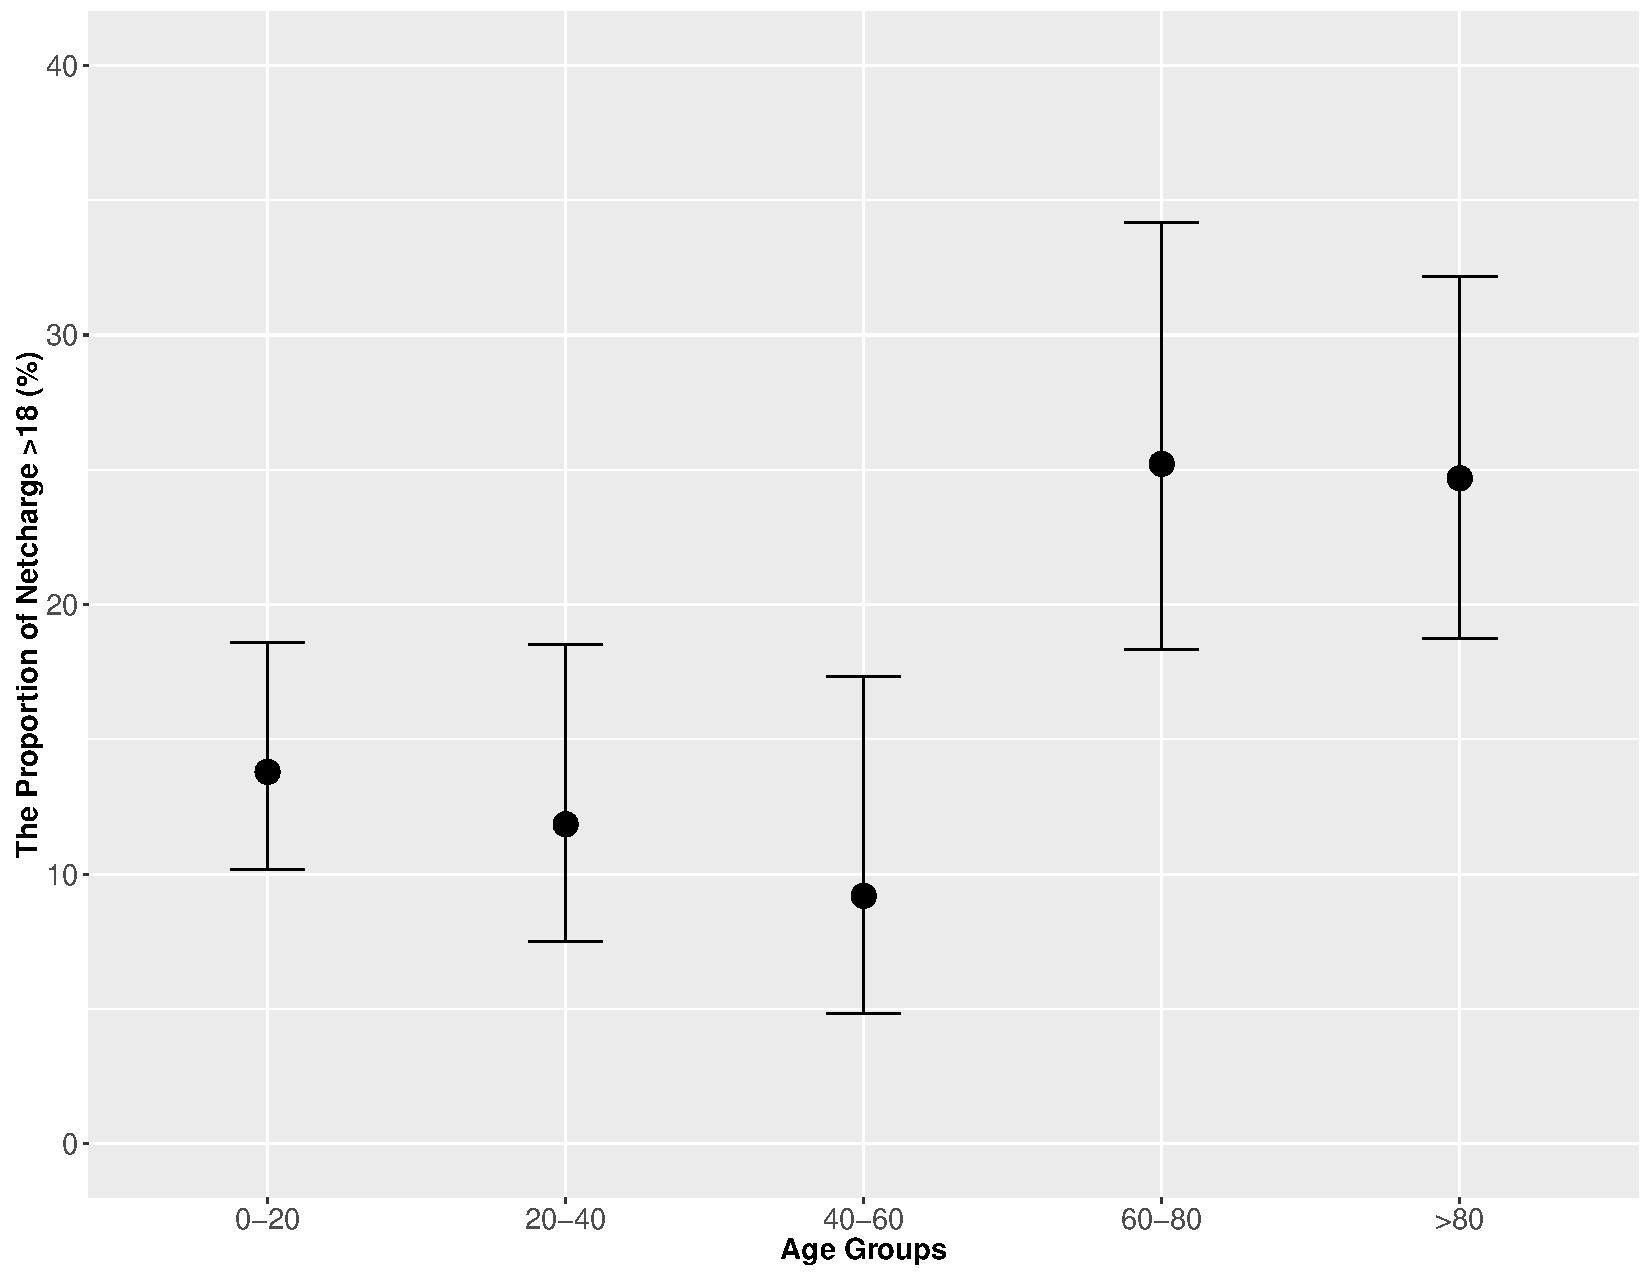
\includegraphics[width=0.6\textwidth]{fig/png/figure3.png}
%\clearpage
%{\bf Figure 4}
%\includegraphics[width=1\textwidth]{fig/png/Figure4.png}
%\clearpage
%{\bf Figure 5}
%\includegraphics[width=1.18\textwidth]{fig/png/Figure5.png}
%\clearpage
%{\bf Figure 6} \\
%\includegraphics[width=0.9\textwidth]{fig/png/figure6.png}
%\clearpage
%{\bf Figure 7}
%\includegraphics[width=1\textwidth]{fig/png/Figure7.png}
%\clearpage
%{\bf Figure 8}
%\includegraphics[width=1.18\textwidth]{fig/png/Figure8.png}
%\clearpage
%{\bf Figure 9} \\
%\includegraphics[width=0.9\textwidth]{fig/png/figure9.png}
%\clearpage


{\bf Supplementary}
\clearpage

\begin{table}
{\bf Table S1.} Comparison of the net charge properties in both internal and external nodes from the reconstructed phylogenetic tree.

\begin{tabular*}{10cm}{rrrrrr}
\hline\hline \\%inserts double horizontal lines

Net charge&  Dec. or Neu. &  Inc. & Total  & \\
\hline \\ %inserts double horizontal lines
$ \geq 0$  &  39          &  10   & 49     &  \\
$ < 0$       &   6           &  19   & 25     &  \\
Total         &  45           &  29   & 74    &  \\
\hline %inserts double horizontal lines
\end{tabular*}
\end{table}
P value = 0.0001 using Fisher's exact test

\clearpage


\begin{table}
{\bf Table S2.} Comparison of the net charge distribution on internal and external nodes of the phylogenetic tree.

\begin{tabular*}{16cm}{rrrrrrr}
\hline\hline \\%inserts double horizontal lines
  & Total strains&  \parbox[c]{1.8 cm}{\raggedright No. strains change netcharge}  &    \parbox[c]{1.8cm}{\raggedright Positive changes} &   \parbox[c]{1.8cm}{\raggedright Negative changes} &     \parbox[c]{1.8cm}{\raggedright Prop High Netcharge}    &     \parbox[c]{1.8cm}{\raggedright Avg netcharge}   \\
\hline \\ %inserts double horizontal lines
Internal &  684 & 53 (7.7\%) &  15 &   38 & 20.0 (\%) & 17.52 $\pm 1.13$\\ \\
External &  686 & 83 (12.1\%) &  32 &   51 & 18.7 (\%)& 17.45 $\pm 1.18$\\ \\
\hline %inserts double horizontal lines
\end{tabular*}
\end{table}
\clearpage

\begin{table}
{\bf S3 Table.} Parameters used in individual based simulation.
\begin{tabular*}{13.5cm}{rrrrr}
\hline\hline \\%inserts double horizontal lines
Parameter names &  symbols &  values &    \\ \\
\hline \\ %inserts double horizontal lines
Total Population  &    $N$ &  1,000,000 &      \\ \\
Birth \& Death rate  & $B$  & 1/(70*365) &   \\ \\
Recovery rate  &  $\gamma$  & 1/3.3 &  \\ \\
Waning rate    &  $\omega$  & 1/25   &  \\ \\
Antibody boosting  & $g$     & 3     &  \\ \\
Initial antigenic mutant & $\Delta A$& 2     & \\ \\
Initial number of seeds & $I_{t=0}$& 10     & \\ \\
Initial virus binding avidity & $V_{0}$& 0.45     & \\ \\
Number of viruses transmitted & $\sigma $ & 1     &  \\ \\
Number of replicated viruses &  $n$       & 4     &  \\ \\
Contact rate &     $c$       & 4     &  \\ \\
Prob of random antigenic mutation & $\psi$  & 0.1     &  \\ \\
Effect of the antigenic mutation &  $\kappa_{a}$       & 0.05     &  \\ \\
Constant of by-product &     $\kappa_{b}$       & 0.01     &  \\ \\
genetic variance &     $V_{c}$       & 0.075     &  \\ \\
\hline %inserts double horizontal lines
\end{tabular*}
\end{table}
\clearpage

{\bf Table S4.} List of all the collected mutations with the corresponding binding avidity (RDE). (Attached as the excel file)
\clearpage



\includegraphics[width=1\textwidth]{fig/png/FigureS1.png}
{\bf FigureS1.} The relative binding avidity by absolute net charge. The value is calculated as the log ratio of RDE activity of the mutant to the wild type. Absolute net charges of all the mutant strains are calculated. Positive correlation is demonstrated with P-value = 0.009 using F-statistic test.
\clearpage
\includegraphics[width=1\textwidth]{fig/png/FigureS2.png}
{\bf FigureS2.}  Comparison of within- and between-host relative fitness at different time during an epidemic. Reds lines represent the average relative fitness within newly infected (immunologically naive) hosts. Blue lines represent effective reproductive number in the human population. Solid lines represent the fitness at day 1 and the dashed lines represent the fitness at day 200 (near the peak).
\clearpage
\includegraphics[width=1\textwidth]{fig/png/FigureS3.png}
{\bf FigureS3.} The neutral effect of within-host binding avidity adaptation on viral phylogeny. Parameter values were as described in Figure3A and C, with contact rate $c=0.3$.
\clearpage
\includegraphics[width=1\textwidth]{fig/png/FigureS4.png}
{\bf FigureS4.}  Schema of the disease transmission in the individual-based model. The status of each individual host during the infection was illustrated. $J$ is the immunity of the host against the challenging virus $v_{i}$. $V$ is the binding avidity and $\delta$ is the antigenic change of the virus. 
\clearpage



\clearpage
\end{document}


